\insertmeeting 
	{Silly Signal Sleeve} 
	{09/20/22}
	{Hagerty High School}
	{Anouska, Mohana, Ritam, Samantha}
	{Images/RobotPics/robot.jpg}
	{2:30 - 4:00}
	
\hhscommittee{Software}
\noindent\hfil\rule{\textwidth}{.4pt}\hfil
\subsubsection*{Goals}
\begin{itemize}
    \item Plan and work on signal sleeve

\end{itemize} 

\noindent\hfil\rule{\textwidth}{.4pt}\hfil

\subsubsection*{Accomplishments}
The signal sleeve is a very valuable part of the autonomous, and considering hardware only needs to make a drivetrain in order to park for it, it serves as a relatively easy and valuable method of scoring, and can give us a great advantage. Even just being able to park in one of the parking areas can give us 20 points one third of the time. But we can certainly do better, and with a lot of time on our hands as we wait for hardware to finish the drive train, it's also the only thing we can really prepare for at the moment.

The current plan for our signal sleeve is to use vision to detect three different colors, green, purple, and gold. We selected these colors because they are colors that do not appear on the field. Colors like gray, red, blue, or yellow are very common and much more likely to trigger the camera and make the robot execute the wrong commands with the wrong randomization. After printing, cutting, and gluing our signal sleeve, we took photos of each side to tune the algorithm on OpenCV. We found that using an HSV threshold was most effective at identifying the colors in the images. In the future, we plan on using this program with a Logitech C270 camera, the one we will be using on our robot, and if that works, it will be ready for implementation on the robot, whenever the drive train gets built.



% \begin{figure}[htp]
% \centering
% 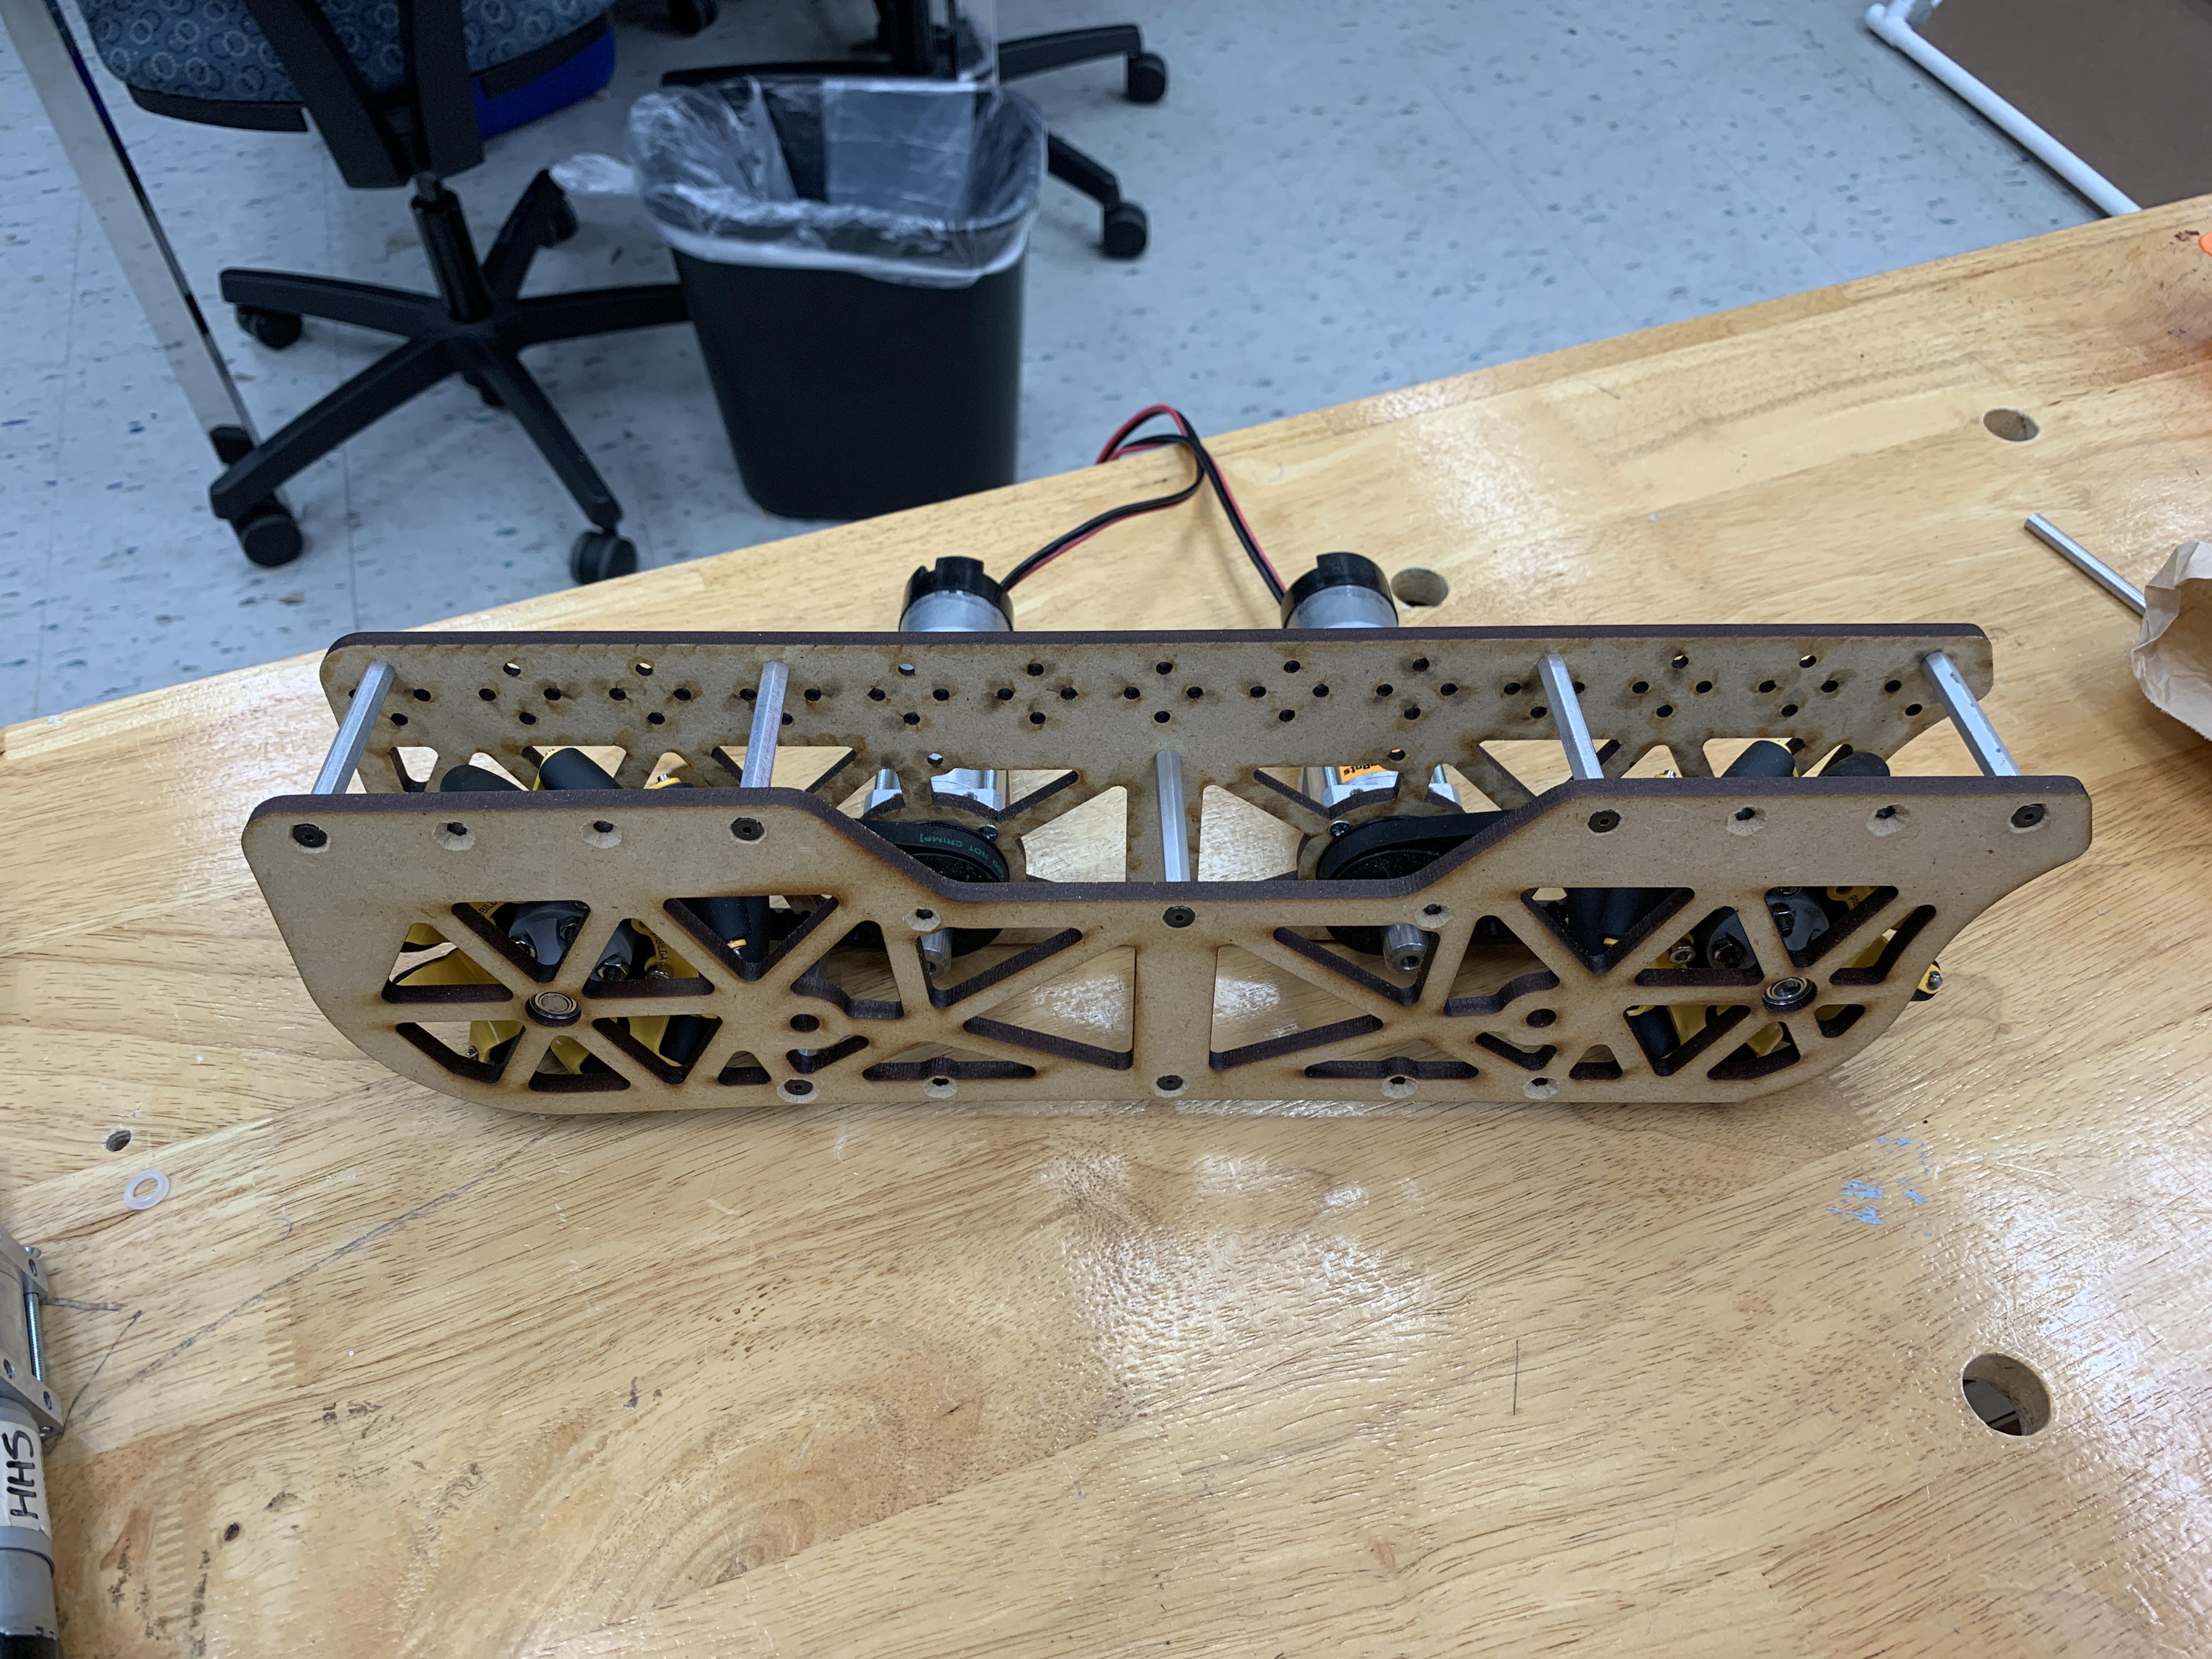
\includegraphics[width=0.9\textwidth, angle=0]{Meetings/July/07-21-21/drivetrain_7-20-21-NathanForrer.jpg}
% \caption{First half of the drivetrain.}
% \label{fig:072121_1}
% \end{figure}

\whatsnext{
\begin{itemize}
    \item Assemble our robot field parts
    \item Continue testing signal sleeve
    \item Reach out to professionals
    
\end{itemize} 
}
